% !TEX encoding = UTF-8 Unicode

A criação do analisador sintático, assim como com o analisador léxico, ocorreu antes da segunda prova e utilizou parte da estrutura criada para o trabalho da disciplina.

A título de recordação, o papel do analisador sintático é obter uma cadeia de tokens proveniente do analisador léxico, e verificar se a mesma pode ser gerada pela gramática da linguagem e, com isso, construir a árvore sintática. Com isso em mente, convertemos a sintaxe da linguagem \emph{SimpPro} para WIRTH, como visto abaixo.

\lstinputlisting[frame=single,breaklines=true,numbers=left]{files/WIRTHorig.txt}

A partir do WIRTH acima, reduzimos a sintaxe para conter somente um autômato, como mostrado abaixo.

\lstinputlisting[frame=single,breaklines=true,numbers=left]{files/WIRTH.txt}

Através de um script, o WIRTH gerado foi então submetido ao site do Hugo Baraúna, seu resultado salvo em arquivos locais, o JFLAP aberto automaticamente e a figura do autômato armazenada localmente, além de gerar automaticamente o pdf impresso para a primeira parte da segunda prova. A Figura~\ref{fig:automato} mostra o autômato final.

\begin{figure}[htbp]
    \centering
    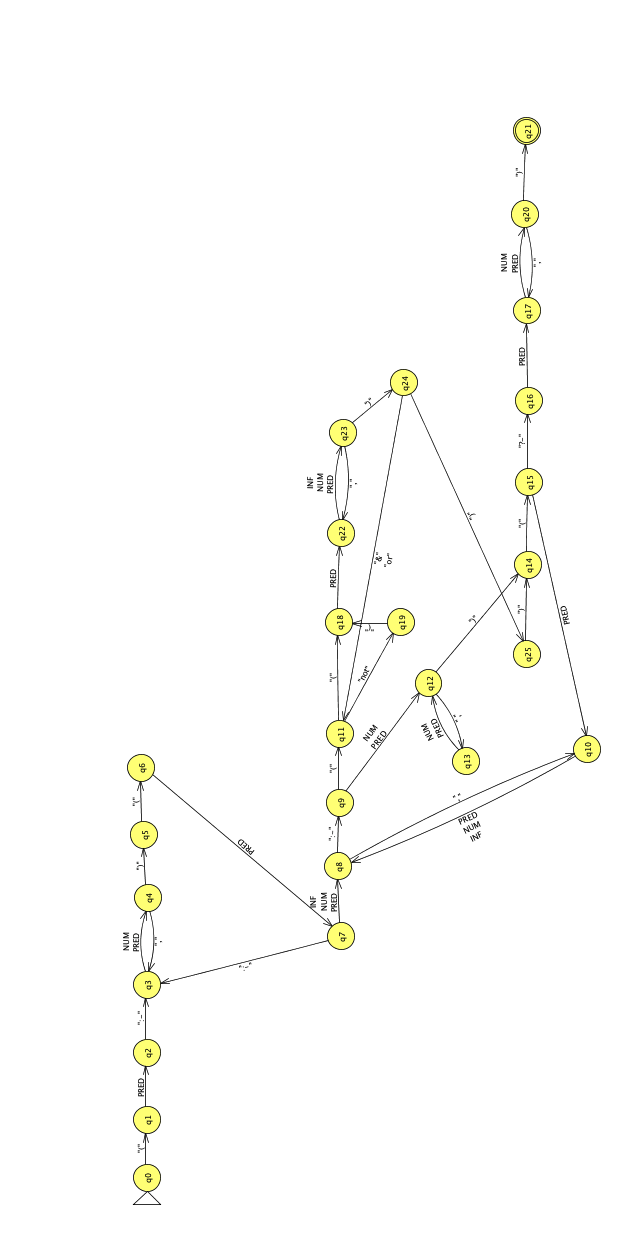
\includegraphics[width=0.75\textwidth]{./images/automato.png}
    \caption{Autômato \emph{Program}}
    \label{fig:automato}
\end{figure}
